% !TeX program = xelatex
% !TeX encoding = UTF-8
% Layout adapted from billryan/resume (MIT); see TEMPLATE-LICENSE.
\documentclass[10pt,a4paper]{article}
\usepackage[top=1.05cm,bottom=1.05cm,left=1.20cm,right=1.20cm,nohead]{geometry}
\usepackage{fontspec}
\usepackage{graphicx}
\usepackage{enumitem}
\usepackage{titlesec}
\usepackage{fontawesome}
\usepackage[hidelinks]{hyperref}
\usepackage{atbegshi}
\pagestyle{empty}
\setlength{\parindent}{0pt}
\setlength{\parskip}{0pt}
\setlength{\emergencystretch}{2em}
\setmainfont{texgyretermes-regular.otf}[BoldFont=texgyretermes-bold.otf,ItalicFont=texgyretermes-italic.otf]
\setsansfont{texgyreheros-regular.otf}[BoldFont=texgyreheros-bold.otf]
\titleformat{\section}{\fontsize{12}{14}\selectfont\raggedright\bfseries}{}{0em}{}[\titlerule]
\titlespacing*{\section}{0pt}{4pt}{2pt}
\titleformat{\subsection}{\normalsize\raggedright}{}{0em}{}
\titlespacing*{\subsection}{0pt}{3pt}{1pt}
\newcommand{\datedsubsection}[2]{\par\addvspace{3pt}\noindent\makebox[\linewidth][l]{\textbf{#1}\hfill{\fontsize{9}{11}\selectfont #2}}\par\nobreak\vspace{1pt}}
\newcommand{\name}[1]{\centerline{\fontsize{22}{25}\selectfont\bfseries #1}\vspace{5pt}}
\newcommand{\email}[1]{\faEnvelope\ \href{mailto:#1}{#1}}
\newcommand{\phone}[1]{\faPhone\ #1}
\newcommand{\basicInfo}[1]{\centerline{\sffamily\fontsize{9.5}{12}\selectfont #1}}
\newcommand{\tech}[1]{{\fontsize{8.9}{10.5}\selectfont\itshape #1\par}\vspace{1pt}}
\setlist[itemize]{label=\textbullet,leftmargin=1.25em,labelsep=0.45em,
  itemsep=0.7pt,topsep=1pt,parsep=0pt,partopsep=0pt}
\newcount\cvpages
\AtBeginShipout{\global\advance\cvpages by 1
  \ifnum\cvpages>1\PackageError{cv}{Resume exceeds one page}{Shorten the content or adjust spacing.}\fi}
\begin{document}
\fontsize{9.2}{11}\selectfont
% Symmetric side columns center the name and contacts independently of the photo.
\noindent\begin{minipage}[c]{0.14\textwidth}
  \rule{0pt}{1.9cm}
\end{minipage}%
\begin{minipage}[c]{0.72\textwidth}
  \name{Xintong Li}
  \basicInfo{\phone{+65 8697 4095}\quad\textperiodcentered\quad\email{xintong.li@u.nus.edu}}
\end{minipage}%
\begin{minipage}[c]{0.14\textwidth}
  \raggedleft
  \IfFileExists{assets/resume_photo.png}{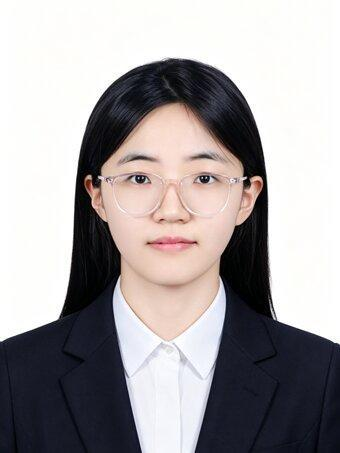
\includegraphics[width=1.5cm]{assets/resume_photo.png}}{\rule{0pt}{1.9cm}}
\end{minipage}\par

\section{\faGraduationCap\ Education}
\datedsubsection{National University of Singapore \quad Master of Computing (MComp)}{Aug 2026 -- Present}
\datedsubsection{Beijing University of Posts and Telecommunications \quad B.Eng., Communication Engineering}{Sep 2022 -- Jun 2026}
Average score: \textbf{90.47/100}; \textbf{top 5\%} of the major. Awarded the \textbf{National Scholarship} and named a \textbf{Beijing Outstanding Graduate}.

\section{\faUsers\ Professional Experience}
\datedsubsection{Kuaishou \quad AI Agent Development Engineer Intern (Code Agent)}{May 2026 -- Jul 2026}
\tech{LangGraph / OpenCode / Context Engineering / Style Memory / Test-Time Scaling}
Contributed to a Code Agent that converts designs into interactive applications, optimizing structured context, task decomposition, designer style memory, and iterative inference for multi-page code generation.
\begin{itemize}
  \item \textbf{Context engineering:} Structured Figma layouts, components, styles, and assets into page-level representations to address redundant node expansion and long multi-page context; loaded relevant information on demand from task workspaces.
  \item \textbf{Hierarchical planning:} Decomposed tasks with LangGraph into individual page implementation, cross-page integration, and interaction/animation completion. Persisted page context and generated artifacts to reuse information across stages and support multi-page generation.
  \item \textbf{Style memory for self-evolution:} Persisted and reused designers' style preferences as conditioning information alongside current design context, supporting cross-task preference accumulation and consistent personalized generation.
  \item \textbf{Test-time scaling:} Connected generation, execution feedback, and iterative repair through OpenCode. Used runtime errors to guide revisions and analyzed sizing, font, and layout failures to refine context construction and generation strategies.
\end{itemize}

\section{\faCode\ Projects}
\datedsubsection{MiniOneRec: Generative Recommendation System \quad Project Lead}{Aug 2026 -- Oct 2026}
\tech{Python / Sentence-BERT / RQ-VAE / Qwen2.5 / SFT / GRPO / DeepSpeed ZeRO-2}
Built an end-to-end framework that compresses item semantics into discrete semantic IDs and uses an LLM for sequence generation and preference alignment, addressing limited semantic transfer in ID-based recommendation.
\begin{itemize}
  \item \textbf{Semantic IDs and constrained decoding:} Encoded item titles and descriptions with Sentence-BERT and quantized embeddings into hierarchical semantic IDs (SIDs) using a three-level RQ-VAE. Applied iterative collision resolution and constrained decoding, achieving \textbf{100\% valid SID generation}.
  \item \textbf{Multi-task supervised fine-tuning:} Converted user interaction histories into SID sequences for Qwen2.5; combined language modeling and SID alignment objectives for next-token prediction. Trained on \textbf{8 A100 GPUs} with DeepSpeed ZeRO-2 to reduce memory usage and accelerate convergence.
  \item \textbf{Recommendation-oriented GRPO:} Optimized the SFT model with a composite reward for hit correctness and ranking quality; used constrained beam search at inference to produce valid, deduplicated recommendation candidates.
  \item \textbf{Results:} On Amazon Industrial \& Scientific, improved \textbf{Recall@10 by 15.2\%} and \textbf{NDCG@10 by 12.8\%} over a traditional ID-based recommendation baseline.
\end{itemize}

\datedsubsection{LLM Agent for Network Fault Root Cause Analysis}{Dec 2025 -- Mar 2026}
\tech{Python / Qwen2.5-7B-Instruct / PEFT / LoRA / GRPO / LangChain / ReAct / RAG}
Combined structured metrics, knowledge retrieval, and multi-step reasoning to diagnose network faults and identify candidate root causes.
\begin{itemize}
  \item \textbf{Two-stage distilled SFT data:} Built \textbf{2,400 examples} from TeleLogs using engineering parameters, observed metrics, symptoms, and candidate causes. Generated traces with exclusion, contradiction, rule-based, and statistical strategies; consolidated and standardized correct traces with a teacher model.
  \item \textbf{Parameter-efficient adaptation:} Fine-tuned Qwen2.5-7B-Instruct with PEFT/LoRA, then applied GRPO to improve root-cause selection and decision consistency in complex fault scenarios.
  \item \textbf{ReAct diagnosis:} Built LangChain tools for table parsing, fault-interval detection, serving-cell geometry, and neighboring-cell interference analysis; combined structured evidence with a rule knowledge base and RAG for interpretable multi-step diagnosis.
  \item \textbf{Results:} Pass@1 increased from 12.04\% (base) to 53.59\% (fine-tuned) and \textbf{76.50\%} (with agent); Pass@4 increased from 12.50\% to 54.86\% and \textbf{78.36\%}, respectively.
\end{itemize}

\datedsubsection{CADDesigner: Agent-Based CAD Model Generation}{Jun 2025 -- Sep 2025}
\tech{Python / LangChain / Claude Sonnet / CadQuery / PythonOCC / ReAct / Function Calling}
Built a text/image-to-CAD pipeline covering code generation, model construction, three-view rendering, and iterative repair for non-expert users.
\begin{itemize}
  \item \textbf{Agentic modeling:} Orchestrated requirement parsing, code generation, model construction, rendering, visual assessment, and iterative repair with LangChain, multi-step reasoning, and tool calls.
  \item \textbf{Multimodal code generation:} Used Claude Sonnet to extract geometric features, structural relationships, and modeling constraints from text and reference images, then generate parametric CadQuery/PythonOCC code.
  \item \textbf{Visual feedback and repair:} Executed code in a sandbox, built 3D models, and rendered standard three-view drawings. Fed visual results back to the agent to revise or regenerate code when outputs differed from requirements.
  \item \textbf{Results:} On CAD-VGDrawing, achieved IoU 0.2769, CD 0.1097, HD 0.4347, and \textbf{100.0\% valid-model generation success (SUC)}.
\end{itemize}

\section{\faCogs\ Skills}
\textbf{Development:} Linux, Shell, Git, Conda, remote GPU servers.\par
\textbf{Model training:} LoRA/QLoRA, PEFT, GRPO; dataset construction, domain adaptation, and evaluation.\par
\textbf{Agents:} LangGraph, LangChain, ReAct, tool calling, multi-agent systems.
\end{document}
